\documentclass[a4paper,twoside]{report}

\usepackage{geometry}
\usepackage{multicol}
\usepackage{caption}
\usepackage{graphicx}
\usepackage{pgf}
\usepackage{multirow}
\usepackage{wrapfig}
\usepackage{indentfirst}
\usepackage{setspace}
\usepackage{amsmath}
\usepackage{mathtools}

\geometry{
	top=2cm,
	bottom=2cm,
	left=2cm,
	right=2cm,
}
\graphicspath{{./img/}}
\setlength{\columnseprule}{1pt}

\newenvironment{Figure}
  {\par\medskip\minipage{\linewidth}}
  {\endminipage\par\medskip}

\begin{document}
    \section*{Part 6}\setlength{\parindent}{0pt}.
        $R = 0\Omega$ : Undamped System \\
        $R = 3000\Omega$ : Oscillatory Damped System \\
        $R = 4671\Omega$ : Critically Damped System \\
        $R = 5500\Omega$ : Over Damped System
        \begin{center}
            \begin{Figure}
                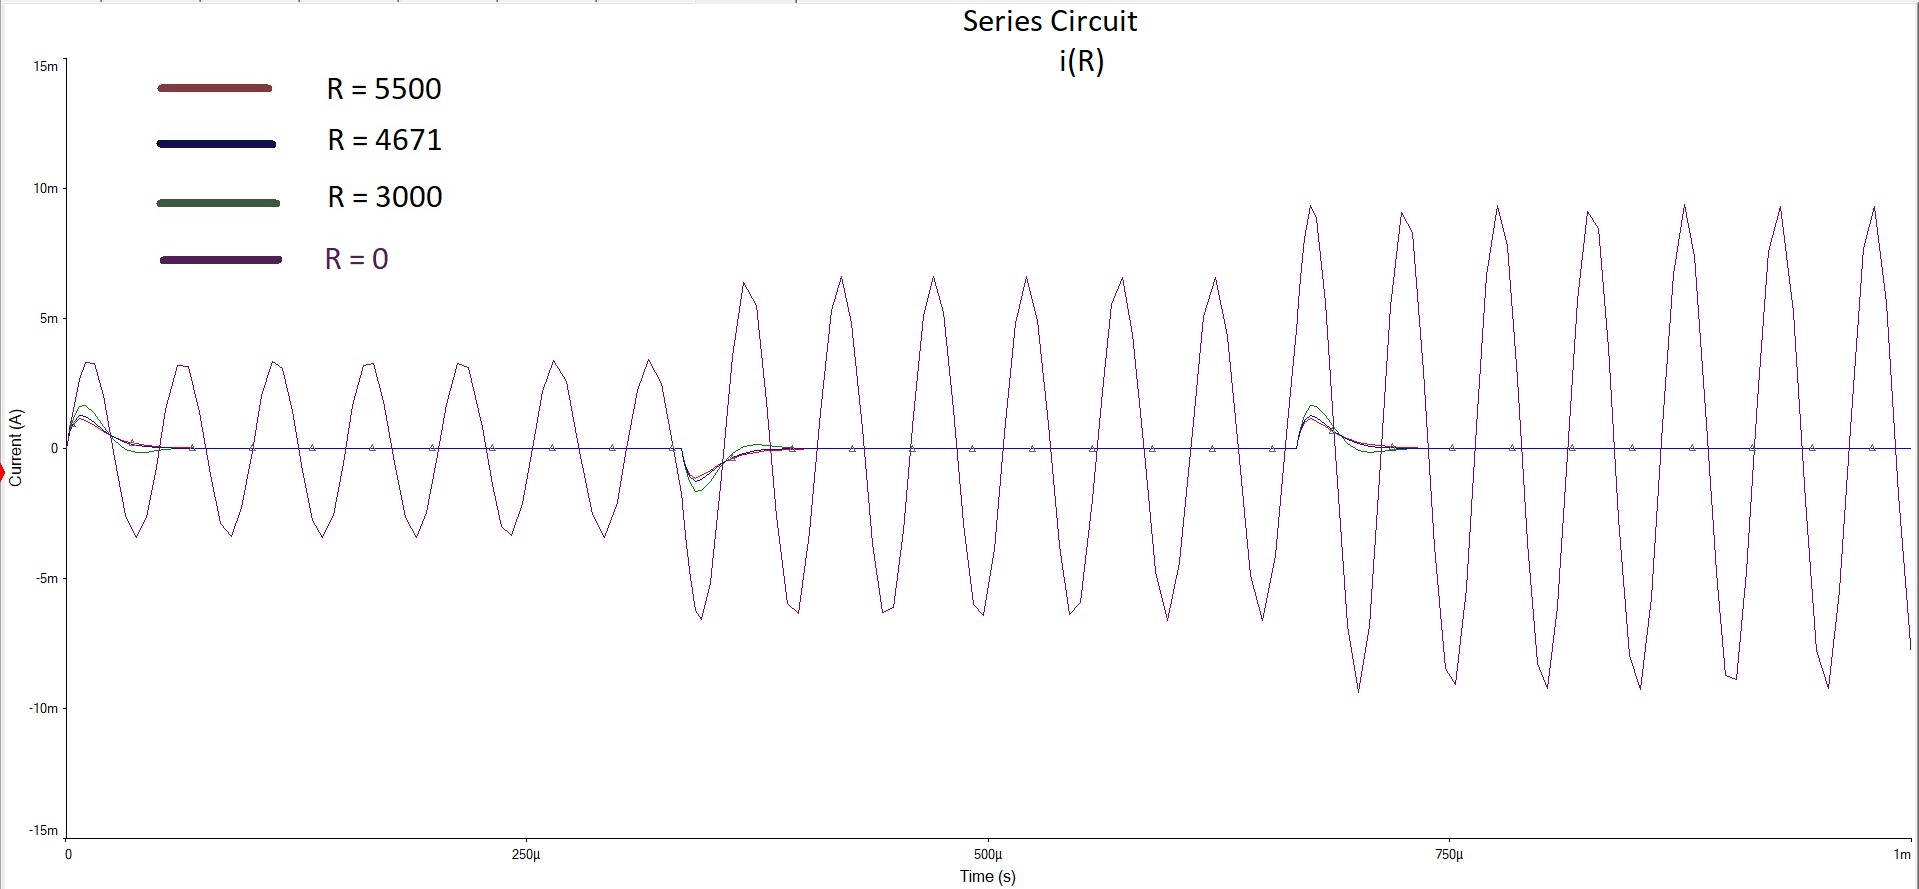
\includegraphics[width=0.8\linewidth]{part6-resistor.jpg}
                \captionof{figure}{Resistor}
            \end{Figure}
            \begin{Figure}
                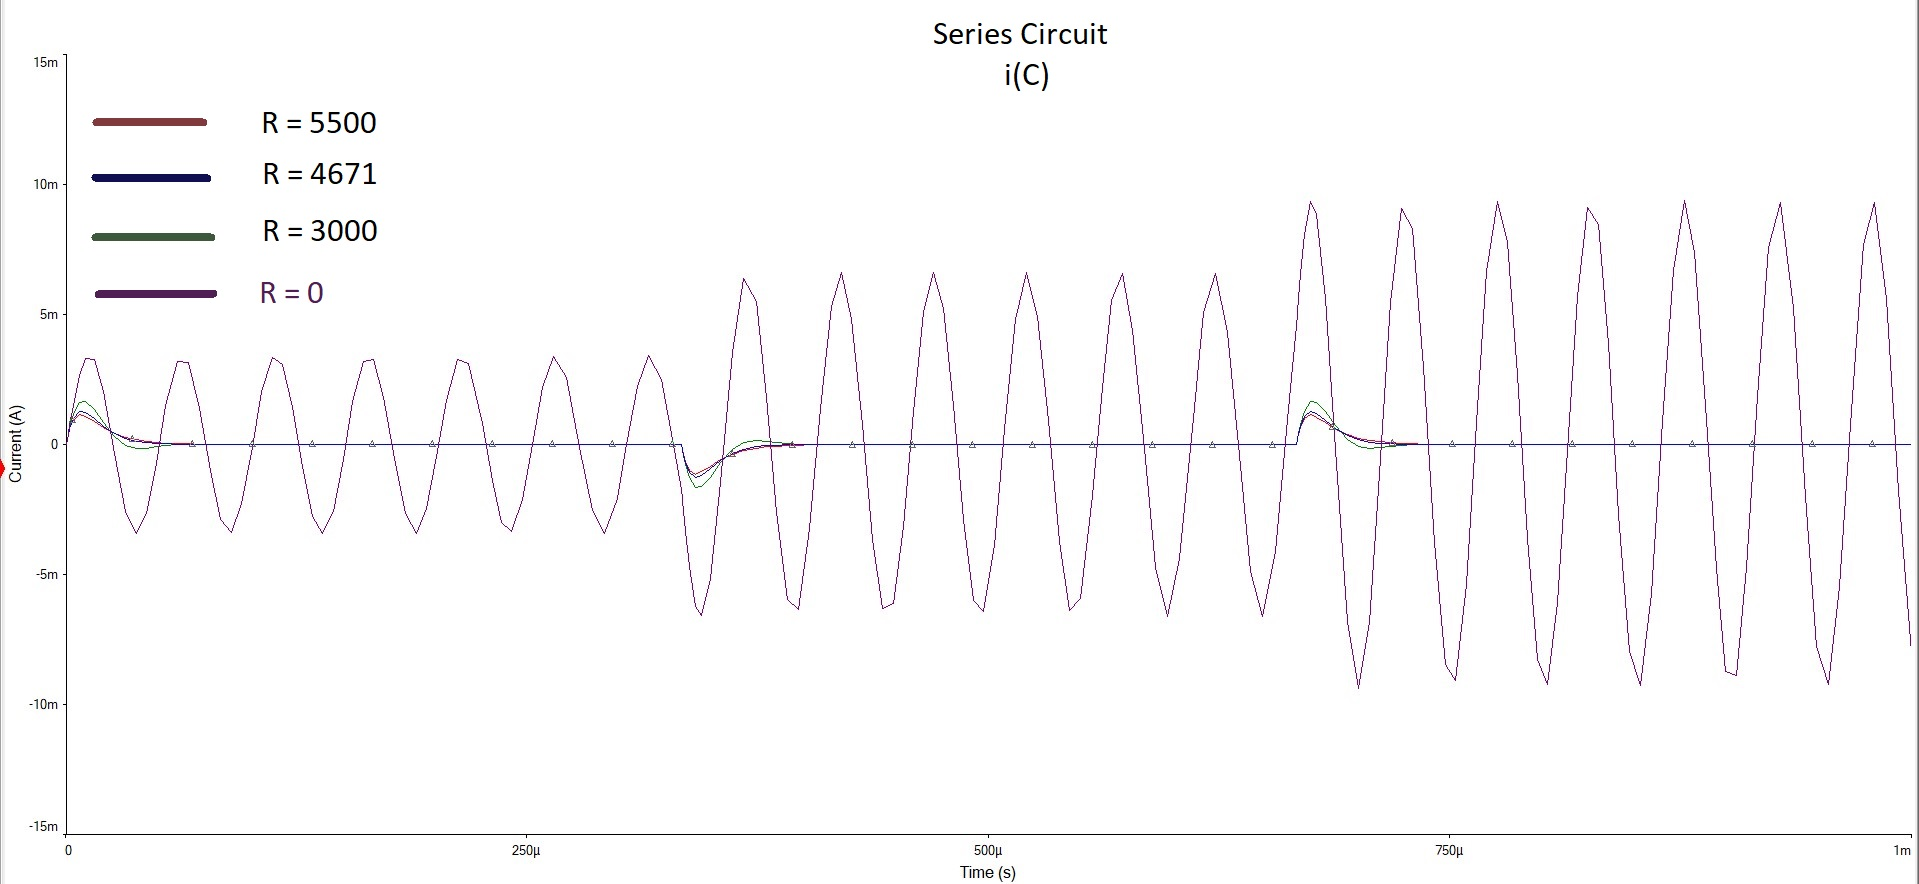
\includegraphics[width=0.8\linewidth]{part6-capacitor.jpg}
                \captionof{figure}{Capacitor}
            \end{Figure}
            \begin{Figure}
                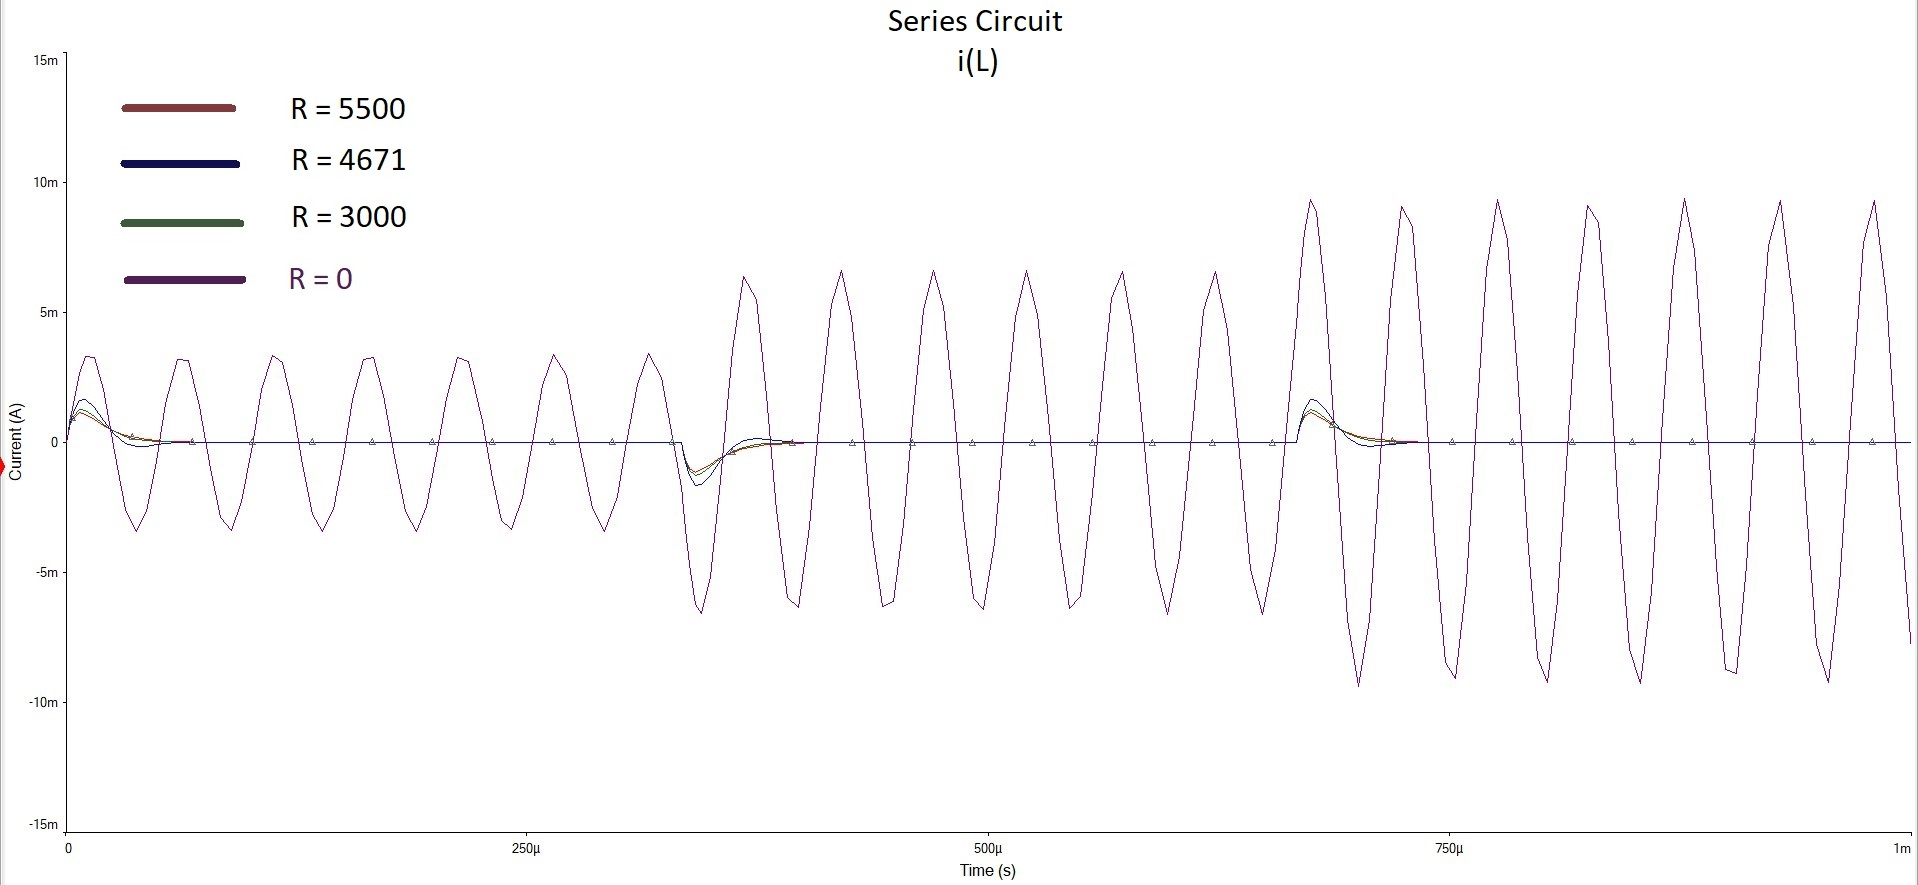
\includegraphics[width=0.8\linewidth]{part6-inductor.jpg}
                \captionof{figure}{Inductor}
            \end{Figure}
        \end{center}
\end{document}
